\documentclass[10pt, c, xcolor=x11names]{beamer}\usepackage[]{graphicx}\usepackage[]{color}
%% maxwidth is the original width if it is less than linewidth
%% otherwise use linewidth (to make sure the graphics do not exceed the margin)
\makeatletter
\def\maxwidth{ %
  \ifdim\Gin@nat@width>\linewidth
    \linewidth
  \else
    \Gin@nat@width
  \fi
}
\makeatother

\definecolor{fgcolor}{rgb}{0.345, 0.345, 0.345}
\newcommand{\hlnum}[1]{\textcolor[rgb]{0.686,0.059,0.569}{#1}}%
\newcommand{\hlstr}[1]{\textcolor[rgb]{0.192,0.494,0.8}{#1}}%
\newcommand{\hlcom}[1]{\textcolor[rgb]{0.678,0.584,0.686}{\textit{#1}}}%
\newcommand{\hlopt}[1]{\textcolor[rgb]{0,0,0}{#1}}%
\newcommand{\hlstd}[1]{\textcolor[rgb]{0.345,0.345,0.345}{#1}}%
\newcommand{\hlkwa}[1]{\textcolor[rgb]{0.161,0.373,0.58}{\textbf{#1}}}%
\newcommand{\hlkwb}[1]{\textcolor[rgb]{0.69,0.353,0.396}{#1}}%
\newcommand{\hlkwc}[1]{\textcolor[rgb]{0.333,0.667,0.333}{#1}}%
\newcommand{\hlkwd}[1]{\textcolor[rgb]{0.737,0.353,0.396}{\textbf{#1}}}%
\let\hlipl\hlkwb

\usepackage{framed}
\makeatletter
\newenvironment{kframe}{%
 \def\at@end@of@kframe{}%
 \ifinner\ifhmode%
  \def\at@end@of@kframe{\end{minipage}}%
  \begin{minipage}{\columnwidth}%
 \fi\fi%
 \def\FrameCommand##1{\hskip\@totalleftmargin \hskip-\fboxsep
 \colorbox{shadecolor}{##1}\hskip-\fboxsep
     % There is no \\@totalrightmargin, so:
     \hskip-\linewidth \hskip-\@totalleftmargin \hskip\columnwidth}%
 \MakeFramed {\advance\hsize-\width
   \@totalleftmargin\z@ \linewidth\hsize
   \@setminipage}}%
 {\par\unskip\endMakeFramed%
 \at@end@of@kframe}
\makeatother

\definecolor{shadecolor}{rgb}{.97, .97, .97}
\definecolor{messagecolor}{rgb}{0, 0, 0}
\definecolor{warningcolor}{rgb}{1, 0, 1}
\definecolor{errorcolor}{rgb}{1, 0, 0}
\newenvironment{knitrout}{}{} % an empty environment to be redefined in TeX

\usepackage{alltt}

\usepackage[backend=bibtex,style=authoryear]{biblatex}
\addbibresource{../chapter/biblio.bib} 

\usepackage{tikz}
\usetikzlibrary{calc,shapes,backgrounds,arrows,automata,shadows,positioning}
\tikzstyle{every state}=[fill=red,draw=none,scale=0.7,font=\small,text=white]
\tikzstyle{every edge}=[-,shorten >=1pt,auto,thin,draw]
\tikzstyle{alertstate}=[fill=bleu]

\newcommand{\invcov}{\bOmega}
\newcommand{\covm}{\bSigma}
\newcommand{\empcov}{\bS_n}
\newcommand{\tildeempcov}{\tilde{\bS}_n}
\newcommand{\barempcov}{\bar{\bS}_n}




% THEME BEAMER

\usetheme{teaching}
\usefonttheme[onlymath]{serif}
\graphicspath{{figures/}}

\usepackage{ulem}
\usepackage{multirow}
\usepackage{tikz}


\pgfdeclareimage[width=.5cm]{computer}{computer.png}

\title{\mytitle}
\subtitle{\mysubtitle}

\author{\small Julien Chiquet, MIA Paris}
\institute{\coauthors}
\date{\place,~\thedate}





\AtBeginSection{
  \begin{frame}<beamer>
    \frametitle{Outline}
    \framesubtitle{\insertpart}
    \tableofcontents[currentsection,currentsubsection, subsectionstyle=show/shaded/hide]  
  \end{frame}
}

\AtBeginSubsection{
  \begin{frame}<beamer>
    \frametitle{Outline}
    \framesubtitle{\insertpart}
    \tableofcontents[currentsection,currentsubsection, subsectionstyle=show/shaded/hide]  
  \end{frame}
}

\AtBeginSubsubsection{
  \begin{frame}<beamer>
    \frametitle{Outline}
    \framesubtitle{\insertpart}
    \tableofcontents[currentsection,currentsubsection, subsectionstyle=show/shaded/hide]  
  \end{frame}
}

\newcommand{\dotitlepage}{%
  \begin{frame}
    \titlepage
    \vfill
    \frontreference
    \vfill
    \includegraphics[width=2cm]{logo_inra} \hfill
    \includegraphics[width=2.5cm]{logo_agroparistech}
  \end{frame}
}

\newcommand{\dotoc}{%
  \begin{frame}
    \frametitle{Outline}
    \tableofcontents[currentsection,sectionstyle=show/show,subsectionstyle=hide]
  \end{frame}
}

\def\mytitle{A multi-attribute Gaussian graphical model for inferring multiscale regulatory networks}
\def\mysubtitle{An application in breast cancer}
\def\coauthors{\normalsize joint work with Martina Sundqvist, Guillem Rigaill \\ (original ideas with C. Ambroise, E. kolazcyk) }
\def\place{Statistiques aux Sommets, Rochebrune}
\def\thedate{2018, March the 29th}

\def\frontreference{
\begin{scriptsize}
 \begin{thebibliography}{99}
    \setbeamertemplate{bibliography item}[article]
    \bibitem[CRS]{CRS} \textcolor{black}{J.C., G. Rigaill, M. Sundqvist},
    \newblock Book on Gene Regulatory Networks: Methods and Protocols, Springer
    \newblock Editors: Guido Sanguinetti, PhD and Vân Anh Huynh-Thu, PhD

  \end{thebibliography}

  \defbeamertemplate{bibliography item}{package}{\pgfuseimage{computer}}
  \setbeamertemplate{bibliography item}[package]

  \smallskip

  \begin{thebibliography}{99}
  \bibitem[multiGGM]{multiGGM} \textcolor{black}{multGGM package, development version on github}
    \newblock \texttt{devtools::install\_github("jchiquet/multGGM/multivarNetwork")}
  \end{thebibliography}
\end{scriptsize}

\begin{tikzpicture}[remember picture,overlay]
  \node [xshift=1cm,yshift=5.5cm] at (current page.south west)    {\includegraphics[height=2cm, keepaspectratio]{martina}};
  \node [xshift=-1cm,yshift=5.5cm] at (current page.south east)    {\includegraphics[height=2cm, keepaspectratio]{guillem}};
\end{tikzpicture}
}
\IfFileExists{upquote.sty}{\usepackage{upquote}}{}
\begin{document}

\dotitlepage

\begin{frame}
  \frametitle{Why multi-attribute networks in genomics?}

  \definecolor{genecolor}{RGB}{94,135,173}
  \begin{tikzpicture}
    \tikzstyle{every state}=[fill=orange!70!white,draw=none,text=white]
      
    \node[state] (dna) at (0,0) {DNA};
    \node[state] (rna) at (4,0) {RNA};
    \node[state] (proteins) at (8,0) {Proteins};
    \node[state] (tf) at (6,-1.2) {TF};
    \node[state] (enzyme) at (9,-2) {Enz.};
    \node[draw=none,text=white,fill=genecolor, scale=0.75] (gene) at (0.5,0.5) {genes};
    
    \path
    (dna) edge [->] node[above] {transcription} (rna) 
    (rna) edge [->] node[above] {translation} (proteins) 
    (dna) edge [loop left,->] node[below=10pt] {replication} (dna) 
    (proteins) edge [->] node {} (tf) 
    (proteins) edge [->] node {} (enzyme) 
    (proteins) edge [loop right, ->] node[above left=10pt] {\textcolor{red}{may bind}} (proteins) 
    (tf) edge [bend left, ->] node[midway] {\textcolor{genecolor}{regulates}} ($(rna.west) -(5mm,0)$)
    (rna) edge [-,line width=2pt,draw=white,bend left] ($(rna.west) -(15mm,0)$)
    (rna) edge [bend left, ->] node {\textcolor{genecolor}{regulates}} ($(rna.west) -(15mm,0)$);
  \end{tikzpicture}    

  \vspace{-.5cm}

  \begin{block}{Data integration}
    \begin{itemize}
    \item  Omic technologies  can  profile  cells at  \alert{different
        levels}: DNA, RNA, protein, chromosomal, and functional.
    \item \alert{multiple} molecular  profiles \alert{combined} on the
      same set of biological samples can be \textit{synergistic}.
    \end{itemize}
  \end{block}
  

  % \vfill

  % \textcolor{mblue!75!black}{Remark}: \textit{a close independent work of Kolar
  %   and Xing appeared late 2012\dots}

\end{frame}

\section{Background on sparse GGM}

\begin{frame}
  \frametitle{\alert{Gaussian} Graphical Model}

  Consider a size-$p$ Gaussian random vector:
  $X\sim\mathcal{N}(\bzr_p,\invcov^{-1})$.

  \begin{itemize}
  \item independence is equivalent to null covariance/correlation
  \item  \alert{  conditional  independence is  equivalent  to  null
      partial covariance/correlation}
    \begin{equation*}
      \label{eq:parcor2invcov}
      \rho_{ij}      =  -\invcov_{ij}      /
      \sqrt{\invcov_{ii} \invcov_{jj}}, \qquad \invcov_{ii}=
      \var(X_i|X_{\backslash \{i,j\}})^{-1}
    \end{equation*}
  \end{itemize}


  \begin{block}{Conditional independence structure}
    \vspace{-.5cm}
    \begin{equation*}
      (i,j)  \notin  \mathcal{E}  \Leftrightarrow  Y_i  \indep  Y_j  |
      Y_{\backslash \{i,j\}} \Leftrightarrow \invcov_{ij} = 0.
    \end{equation*}
  \end{block}

  \vspace{-.5cm}
  \begin{block}{Graphical interpretation}
    \vspace{-.5cm}
    \begin{center}
      \begin{tabular}{c@{\hspace{2cm}}c}
        \begin{tabular}{c}
          \small $\mathcal{G}=(\mathcal{P},\mathcal{E})$ \\
          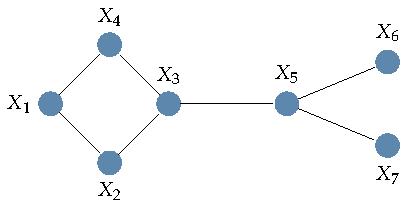
\includegraphics[width=.3\textwidth]{graph}
        \end{tabular}
     &
       \begin{tabular}{c}
         \small $\invcov$\\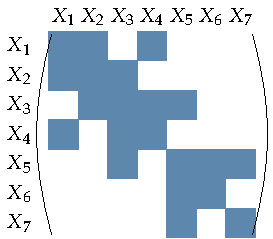
\includegraphics[width=.2\textwidth]{Markovadjacency}
       \end{tabular}
      \end{tabular}
    \end{center}
  \end{block}
  \vspace{-.5cm}

  \rsa Network reconstruction is (roughly) a variable selection problem
\end{frame}

\begin{frame}
  \frametitle{Gaussian Graphical Model and Linear Regression}

  \begin{block}{Linear regression viewpoint}
    Gene expression $X_j$ is linearly explained by the other genes':

    \begin{equation*}
      X_j | X_{ \setminus j} = - \sum_{k \neq j}
      \frac{\invcov_{jk}}{\invcov_{jj}} X_{k} + \varepsilon_j,\quad \varepsilon_j
      \sim \mathcal{N}(0,\invcov_{jj}^{-1}), \quad \varepsilon_j \perp X_j
      \end{equation*}
      Conditional  on its  neighborhood,  other profiles  do not  give additional insights
    \begin{equation*}
      X_j | X_{ \setminus j} =
       \sum_{k \in \text{ne(j)}} \beta_{jk} X_k + \varepsilon_j
      \quad         \text{with         }         \beta_{jk}         =
      -\frac{\invcov_{jk}}{\invcov_{jj}}.
    \end{equation*}
  \end{block}

  % \vspace{-.5cm}
  % \begin{overlayarea}{\textwidth}{.45\textheight}
  %   \begin{block}{Graphical Interpretation}
  %     \vspace{-.5cm}
  %     \begin{center}
  %       \begin{scriptsize}
  %         \begin{tabular}{cc}
  %           Local Markov property & Global Markov property \\
  %           conditioning on the neighborhood & conditioning on a separating node\\
  %           \includegraphics[width=.4\textwidth]{localMarkov}
  %           & \includegraphics[width=.4\textwidth]{globalMarkov}\\
  %         \end{tabular}
  %       \end{scriptsize}
  %     \end{center}
  %   \end{block}
  % \end{overlayarea}

  \vfill
  \alert{$\rightsquigarrow$ ``Neighborhood'' selection}

\end{frame}

\begin{frame}
  \frametitle{Gold standard penalized approaches}
  \framesubtitle{Use $\ell_1$ for both regularizing and promoting \textit{sparsity}}

  \begin{overlayarea}{\textwidth}{\textheight}

    \begin{block}{Penalized   likelihood  (Banerjee   \textit{et
          al.}, Yuan and Lin, 2008)}
      \vspace{-1em}
\begin{equation*}
  \label{eq:MLE_l1}
  \widehat{\invcov}^{\text{glasso}}_\lambda = \arg \max_{\invcov \in \mathcal{S}^+_p} \; \log
  \det(\invcov) - \trace{\invcov \empcov} -
  \lambda\ \|\invcov\|_{\ell_1}.
\end{equation*}
    \end{block}
    \vspace*{-1.5em}

    \begin{itemize}
    \item[\textcolor{green}{$+$}] symmetric, positive-definite
    \item[\textcolor{red}{$-$}]       solved      by       the
      ``Graphical-Lasso''                 ($\mathcal{O}(p^3)$,
      \textit{Friedman et al, 2007}).
    \item \texttt{R}-packages \textbf{glasso}, \textbf{quic}, \textbf{huge}.
    \end{itemize}

    \vfill

    \begin{block}{Neighborhood    Selection   (Meinshausen    \&
        B\"ulhman, 2006)}<2-> \vspace*{-1em}
\begin{equation*}
  \label{eq:MB_pseudo}
  \hat\bB^{\text{ns}}  = \argmin_{\bB\in\Rset^{p\times  p}, \diag(\bB)
    =    \bzr_p}    \frac{1}{2}    \trace{\bB^\top\empcov    \bB}    -
  \trace{\bB^\top\empcov} + \lambda \|\bB\|_{\ell_1}.
\end{equation*}
      \vspace*{-1.5em}
    \end{block}

    \onslide<2>{
      \begin{itemize}
      \item[\textcolor{red}{$-$}]     not     symmetric,     not
        positive-definite
      \item[\textcolor{green}{$+$}]   $p$   Lasso  solved   with
        Lars-like   algorithms   ($\mathcal{O}(npd)$   for   $d$
        neighbors).
      \item \texttt{R}-package \textbf{huge}.
      \end{itemize}
    }

\end{overlayarea}

\end{frame}

\begin{frame}
  \frametitle{Gold standard penalized approaches (2)}
  \framesubtitle{Use $\ell_1$ for both regularizing and promoting \textit{sparsity}}

  \begin{overlayarea}{\textwidth}{\textheight}

    \begin{block}{CLIME -- Pseudo-likelihood  (Cai et al., 2011;
        Yuan, 2010)}<1->
      \vspace*{-1.5em}
      \begin{equation*}
        \widehat{\invcov}^{\text{clime}}_\lambda  = \argmin_{\invcov}
        \left\|   \invcov \right\|_1 \text{ subjected to }
        \left\|   \empcov \invcov - \mathbf{I} \right\|_\infty\leq \lambda
      \end{equation*}
      \vspace*{-1.5em}
    \end{block}

    \begin{itemize}
    \item[\textcolor{red}{$-$}] not positive-definite
    \item[\textcolor{green}{$+$}]  $p$ linear  programs easily
      distributed ($\mathcal{O}(p^2d)$ for $d$ neighbors).
    \item \texttt{R}-package \textbf{fastclime} (dedictated imp. up to p=6!).
    \end{itemize}

      \vspace*{-.5em}

    \begin{block}{Sparse PArtial  Correlation Estimation (SPACE)
        (Peng 2009; Khare 2014 )}<2->
      \vspace*{-2em}
      \begin{equation*}
        \left(\widehat{\boldsymbol\rho}_\lambda^{\text{space}}, \mathrm{diag}({\boldsymbol\invcov})\right) =
        \argmin_{\boldsymbol\rho,\mathrm{diag}({\boldsymbol\invcov})} \frac{1}{2}
        \sum_{j=1}^p \omega_j \left\|
          \bx_j - \sum_{k=1}^p \rho_{jk} \sqrt{\frac{{\invcov}_{kk}}{{\invcov}_{jj}}}
          \bx_k \right\|_{\ell_2}^2 + \lambda\ \| \boldsymbol\rho \|_{\ell_1}
      \end{equation*}
      \vspace*{-1.5em}
    \end{block}

    \onslide<2>{
      \begin{itemize}
      \item[\textcolor{green}{$+$}]  for  fixed variances,  same
        cost as neighborhood selection.
      \item[\textcolor{red}{$-$}]    alternate    procedure    without
        guarantees on the number of iterates
      \item \texttt{R}-package \textbf{gconcord}.
      \end{itemize}
    }

\end{overlayarea}

\end{frame}

\begin{frame}
  \frametitle{Practical implications of theoretical results}

  \begin{block}{Selection    consistency    (Ravikumar,    Wainwright,
      2009-2012)}<1->                                           Denote
    $d=\max_{j\in\mathcal{P}}(\mathrm{degree_j})$.  Consistency for an
    appropriate $\lambda$ and
    \begin{itemize}
    \item  $n\approx\mathcal{O}(d^2\log(p))$ for  the graphical  Lasso
      and Clime.
    \item $n\approx\mathcal{O}(d\log(p))$  for   neighborhood
      selection (sharp).
    \end{itemize}
    \textit{(Irrepresentability) conditions are not strictly
    comparable\dots}
  \end{block}

  \vfill

  \begin{block}{Ultra high-dimension phenomenon (Verzelen,  2011)}
    Minimax risk for sparse regression with $d$-sparse models: useless
    when
    \begin{equation*}
    \frac{d \log(p/d)}{n} \geq 1/2, \qquad (\mathrm{e.g.}, n=50, p=200, d\geq 8).
    \end{equation*}
    \textit{Good news! when $n$ is small, we don't need to solve
      huge problems because they can't but fail.}
  \end{block}

\end{frame}

\begin{frame}
  \frametitle{Model selection}

  \begin{block}{Cross-validation}
    Optimal in terms of \alert{prediction}, not in terms of selection
  \end{block}

  \begin{block}{Information based criteria}
    \begin{itemize}
    \item GGMSelect (Girault \textit{et al}, '12) selects among a family of candidates.
    \item Adapt IC to sparse high dimensional problems, e.g.
    \begin{equation*}
      \text{EBIC}_\gamma(\widehat{{\boldsymbol\invcov}}_\lambda)  =   -2 \textrm{loglik}
      (\widehat{{\boldsymbol\invcov}}_\lambda;\bX) + |\mathcal{E}_\lambda| (\log(n) + 4 \gamma \log(p) ).
    \end{equation*}
    \end{itemize}
  \end{block}

  \begin{block}{Resampling/subsampling}
    \alert{Keep edges frequently selected} on an range of $\lambda$ after sub-samplings
    \begin{itemize}
    \item Stability Selection (Meinshausen and B\"uhlman, 2010, Bach 2008)
    \item Stability approach to Regularization Selection (StaRS) (Liu, 2010).
    \end{itemize}
  \end{block}
\end{frame}






\section{Sparse multi-attribute GGM}

\begin{frame}
  \frametitle{Multiattribute GGM}

    Consider e.g. some $p$ genes of interest and the $K=2$ omic experiments
    \begin{enumerate}
    \item $X_{i1}$ is the expression profile of gene $i$ (transcriptomic data),
    \item $X_{i2}$ is the corresponding protein concentration (proteomic data).
    \end{enumerate}

    \vfill

  \begin{block}{Define a block-wise precision matrix}
      \vspace{-.25cm}
      \begin{itemize}
      \item  $X =  (X_1,  \dots,  X_p)^T \sim  \mathcal{N}(\mathbf{0},
        \bSigma)$ in $\Rset^{pK}$,
      \item $X_i=(X_{i1},\dots,X_{iK})^\intercal \in \mathbb{R}^K$.
      \end{itemize}
      \[
      \invcov = \bSigma^{-1} = \begin{bmatrix}
        \invcov_{11} & & \invcov_{1p} \\
        & \ddots & \\
        \invcov_{p1} & & \invcov_{pp} \\
      \end{bmatrix}, \qquad  \invcov_{ij} \in \mathcal{M}_{K,K},
      \ \forall (i,j)\in\mathcal{P}^2.
      \]
    \end{block}

    \vfill

    \begin{beamerboxesrounded}[upper=sur:head,lower=sur:bloc,shadow=true]{Graphical Interpretation}
      Define  $\mathcal{G}=(\mathcal{P},\mathcal{E})$   as  \alert{the
        multivariate analogue} of the {\it conditional graph}:
      \vspace{-.25cm}
      \begin{equation*}
        (i,j)\in    \mathcal{E}    \Leftrightarrow    \invcov_{ij}    \ne
        \mathbf{0}_{KK}.
      \end{equation*}
    \end{beamerboxesrounded}

\end{frame}

\begin{frame}
  \frametitle{Multiattribute GGM as multivariate regression}

  \begin{block}{Multivariate analysis view point}
    Straightforward algebra and we have
    \begin{equation*}
      \label{eq:condK}
      X_j \, |\,  X_{\backslash j}  = x \sim  \mathcal{N}(- \invcov_{jj}^{-1}\invcov_{j
        \backslash j} x , \invcov_{ii}^{-1})\enskip.
    \end{equation*}
    or   equivalently,    letting   $\displaystyle    \mathbf{B}_j^T   =
    -\invcov_{jj}^{-1} \invcov_{i\backslash j}$,
    \begin{equation*}
      \label{eq:condK}
      X_j \, |\, X_{\backslash j} = \mathbf{B}_j^T X_{\backslash j} +
      \boldsymbol\varepsilon_j \quad \boldsymbol\varepsilon_j
      \sim \mathcal{N}(\mathbf{0},\invcov_{ii}^{-1}), \quad \boldsymbol\varepsilon_j \perp X.
    \end{equation*}
  \end{block}

    \begin{colormixin}{60!white}
      \begin{block}{Remembering the univariate case?}
        \[
        X_j   |    X_{   \setminus    j}   =   -    \sum_{\alert{k   \in
            \text{neighbors}(j)}} \frac{\invcov_{jk}}{\invcov{jj}}  X_j +
        \varepsilon_j,\quad              \varepsilon_j              \sim
        \mathcal{N}(0,\invcov_{jj}^{-1}), \quad \varepsilon_j \perp X.
        \]
      \end{block}
    \end{colormixin}
\end{frame}

\begin{frame}
  \frametitle{A matter of notation\dots I}
  \framesubtitle{Matrix of regression coefficients}
  
 $\mathbf{B}_j\in\mathcal{M}_{(p-1)K,K}$ is defined block-wise
  \begin{equation*}
  \mathbf{B}_j = \begin{bmatrix}
    \mathbf{B}_j^{(1)} \\ \hline
    \vdots \\ \hline
    \mathbf{B}_j^{(j-1)} \\ 
    \mathbf{B}_j^{(j+1)} \\ 
    \vdots \\ \hline
    \mathbf{B}_j^{(p)} \\ 
  \end{bmatrix} = - \begin{bmatrix}
    \invcov_{j1} \\ \hline
    \vdots \\ \hline
    \invcov_{j(j-1)} \\ 
    \invcov_{j(j+1)} \\ 
    \vdots \\ \hline
    \invcov_{j(p)} \\ 
  \end{bmatrix}^\top \times \invcov_{jj}^{-1},
\end{equation*}
 \rsa the $K\times K$  matrix  $\mathbf{B}_j^{(i)}$ links attributes of variables $(i,j)$.

\end{frame}

\begin{frame}
  \frametitle{A matter of notation\dots II}
  \framesubtitle{Data matrix}

  Consider an i.i.d.  sample $\{X^\ell\}_{\ell=1}^n$ of $X$ such that
   each attribute is observed $n$ times for the $p$ variables

  \begin{itemize}
    \item $\bx^\ell$ is a $pK$-size row vector
    \item $\bX_j \in \mathcal{M}_{n,K}$ contains the data related to variable $j$ 
    \item $\bX$ is the full data matrix in $\mathcal{M}_{n,pK}$
  \end{itemize}

\begin{multline*}
  \mathbf{X} = \begin{bmatrix}
    \mathbf{x}^1 \\ \hline
    \vdots \\\hline
    \mathbf{x}^n \\
  \end{bmatrix}
  = \begin{bmatrix}
    \mathbf{X}_1 & \dots & \mathbf{X}_p \\
  \end{bmatrix} \\
  = \begin{bmatrix}
    X_{11}^1 & \dots & X_{1K}^1 & \vline & \dots & \vline & X_{p1}^1 & \dots & X_{pK}^1 \\ \hline
    \vdots & & \vdots & \vline & \dots & \vline & & & \\ \hline
    X_{11}^n & \dots & X_{1K}^n & \vline & \dots & \vline & X_{p1}^n & \dots & X_{pK}^n \\ 
  \end{bmatrix}.
\end{multline*}
\end{frame}

\begin{frame}
  \frametitle{Multivariate neighborhood selection} 

  \begin{block}{The penalized multivariate regression approach}
    For each node /gene, recover its neighborhood by solving 
    \begin{equation*}
      \arg  \min_{\mathbf{B}_j  \in  \mathcal{M}_{(p-1)K,K}}  \frac{1}{2n} \left\|
        \bX_j - \bX_{\backslash j}\bB_j\right\|_F^2 +
      \lambda \ \text{Pen}(\bB_j),
    \end{equation*}
  \end{block}
  
  \vfill
  
  \begin{block}{Choice of penalty}
    Group-based   penalty   to   activate  the   set   of   attributes
    simultaneously on a given link:
    \begin{equation*}
      \text{Pen}(\bB_j) =       \sum_{k \neq j}  \|\bB_j^{(k)}\|  \enskip  ,
      \quad \bB_j^{(k)} \in \mathcal{M}_{KK}
    \end{equation*}
    \begin{itemize}
    \item  \alert{$\|M\|=   \|M\|_F=\left(  \sum_{i,j}  M_{ij}^2\right)^{1/2}$,
        the Frobenius norm},
    \item  $\|M\|=  \|M\|_\infty=  \max_{i,j}{|M_{ij}|}$, the  sup  norm
      (shared magnitude),
    \item $\|M\|= \|M\|_\star=\sum \mathrm{eig}(M)$, the nuclear norm
      (rank penalty).
    \end{itemize}      
  \end{block}
\end{frame}



\section{Numerical experiments}

\begin{frame}
  \frametitle{Simulation study: settings}

  \begin{enumerate}
\item  Draw a $p \times p$ adjacency matrix $\bA$ under Erd\"os-Renyi model.
\item  Expand $\bA$  to  multivariate space: 
  $$\mathbf{M} = \mathbf{A}  \otimes \mathbb{S} + \mathbf{I}_{p\times K}$$
  \paragraph{$\mathbb{S}$ is used to consider different scenarios of agreement}
  \begin{enumerate}[a)]
  \item $\mathbb{S} = \mathbf{I}_{K,K}$ \\ 
    \rsa same intra-attribute network, no inter-attribute interactions
  \item $\mathbb{S} = \mathbf{I}_{K,K} - \mathbf{1}_{K,K}$ \\ 
  \rsa same inter-attribute interactions and no intra-attribute interactions
  \item $\mathbb{S} = \mathbf{1}_{K,K}$ \\
    \rsa full agreement between  attributes.
  \end{enumerate}
\item $\invcov$ is the nearest a positive definite approximation of $\mathbf{M}$
\item Control the difficulty with $\gamma>0: \invcov= \invcov+ \gamma I$;
\item Draw an i.i.d. $n$-size sample $\bX\in\Rset^{n\times pK}$ of
  $X \sim \mathcal{N} \left( 0,\invcov^{-1} \right) .$
\end{enumerate}


\end{frame}

\begin{frame}
  \frametitle{Simulation study: evaluation}

  \begin{block}{Competitors}  
  \begin{itemize}
  \item \texttt{multiattribute}: reconstruct one network with
   $K$ data sets $\bX^{(1)}, \dots \bX^{(K)}$ all with size
  $\Rset^{n\times p}$

  \item \texttt{separate}: reconstruct $K$ networks with
   $K$ data sets $\bX^{(1)}, \dots \bX^{(K)}$ all with size
  $\Rset^{n\times p}$

  \item the \texttt{merge} variant: reconstruct one network 
    by merging $\bX^{(1)}, \dots \bX^{(K)}$ into a single
    $\tilde\bX$ data set in $\Rset^{nK \times p}$
  \end{itemize}
  \end{block}
  
  \begin{block}{Performances}  
    Use area under ROC curve (AUC). For the \textit{separate} variant, the retained AUC is the AUC
    averaged over all attributes.  
  \end{block}

  \rsa Set $p=40$, vary $n, K$ and replicate 100 times

\end{frame}


\begin{frame}
  \frametitle{Simulation study: results}
  
  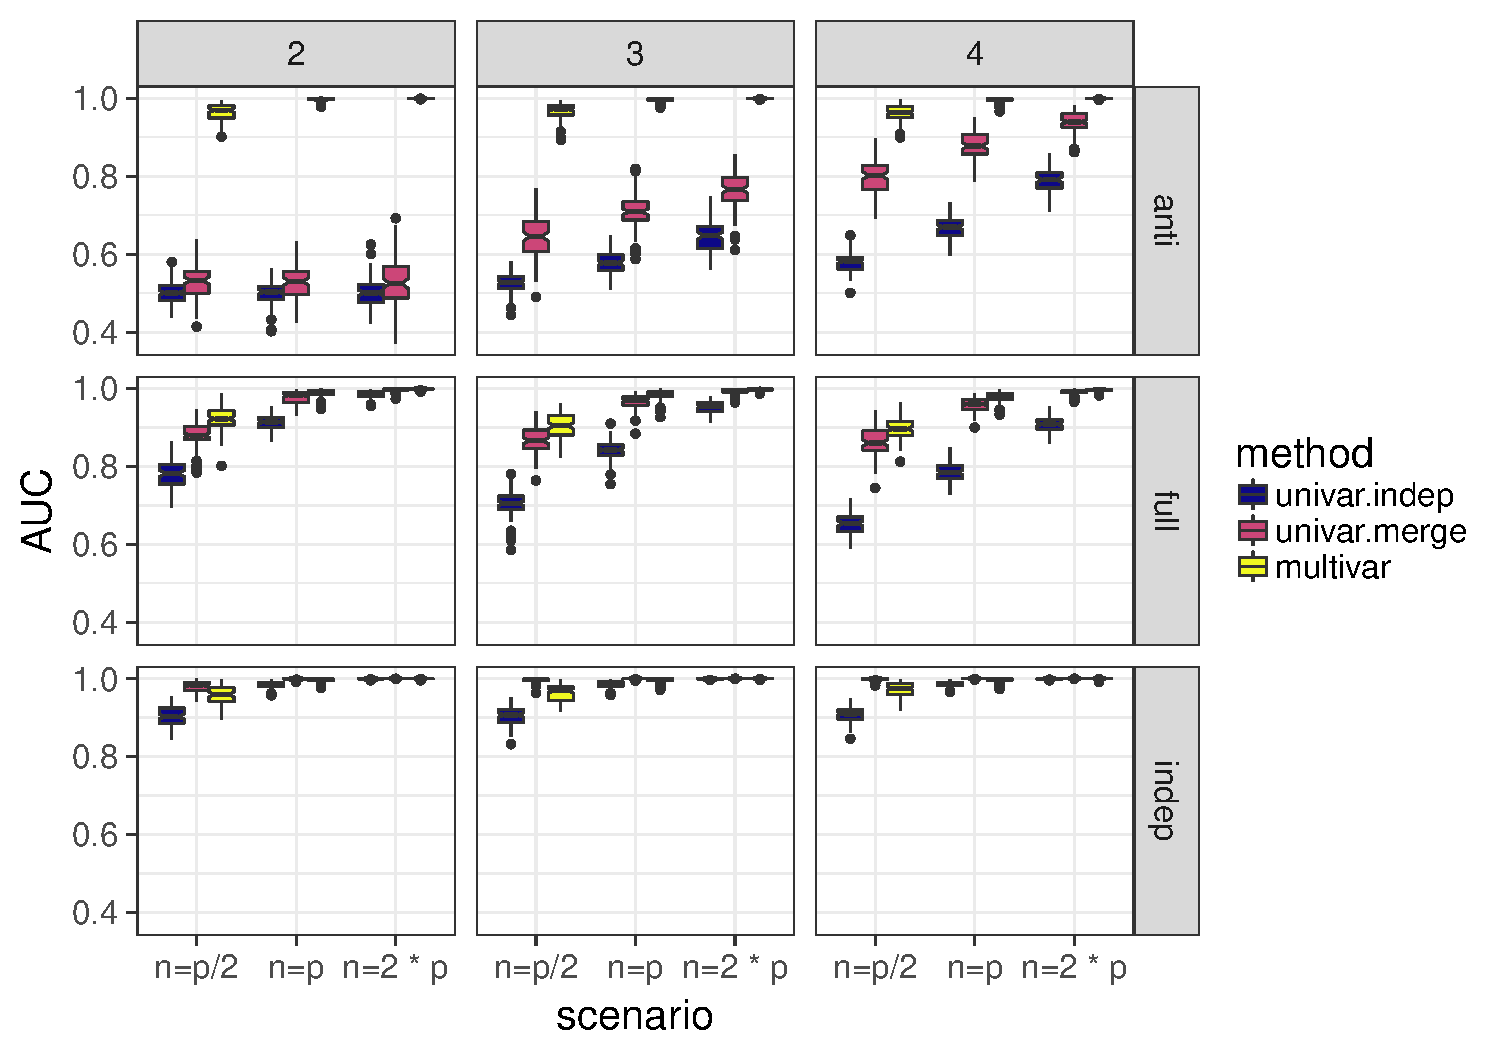
\includegraphics[width=\textwidth]{../../chapter/figures/res_simu_new}

\end{frame}


\paragraph*{Illustration: Gene/Protein regulatory network inference.}

As an illustration, we applied our sparse multiattribute GGM approach
to reconstruct networks on two large breast cancer data sets from the
National Cancer Institute\footnote{\url{https://www.cancer.gov/}} and
the Rational Therapy for Breast Cancer
consortium\footnote{\url{http://www.ratherproject.com/}}, respectively
referred to as NCI-60 and RATHER hereafter. These data sets contain
both proteomic and transcriptomic profiles, respectively measured with
reverse-phase protein arrays (RPPA) and RNA affymetrix array. We infer
the multiattribute network between the subset of molecular entities
which is common to the proteins measured by RPPA and the genes
measured by RNA array, that we call the \textit{consensus set}: in the
NCI-60 cancer line data set \citep{pfister2009topoisomerase}, a
consensus set composed of $p=91$ protein and corresponding gene
profiles is retained, for the $n=60$ samples. The RATHER data set
\citep{michaut2016integration} contains proteomic and transcriptonic
data from $n=100$ patients for a consensus set of $p=117$
entities\footnote{The data can be downloaded from
  \url{https://www.ncbi.nlm.nih.gov/geo/query/acc.cgi?acc=GSE66647}.}.

We infer a sparse GGM for each attribute (gene expression and protein
profile), separately to start with, and then get its multiattribute
version.  We do this on a large grid of the tuning parameter and thus
have three families of networks indexed by their number of edges.

Figure \ref{fig:jaccard} demonstrates that our sparse multiattribute
method captures the characteristics of both univariate networks, as
the Jaccard similarity index is high between each uni-attribute
network and the multiattribute network, while it remains low when
comparing uni-attribute networks together.
\begin{figure}[htbp!]
  \centering
  \begin{tabular}{@{}cc@{}}
   RATHER & NCI-60 \\
    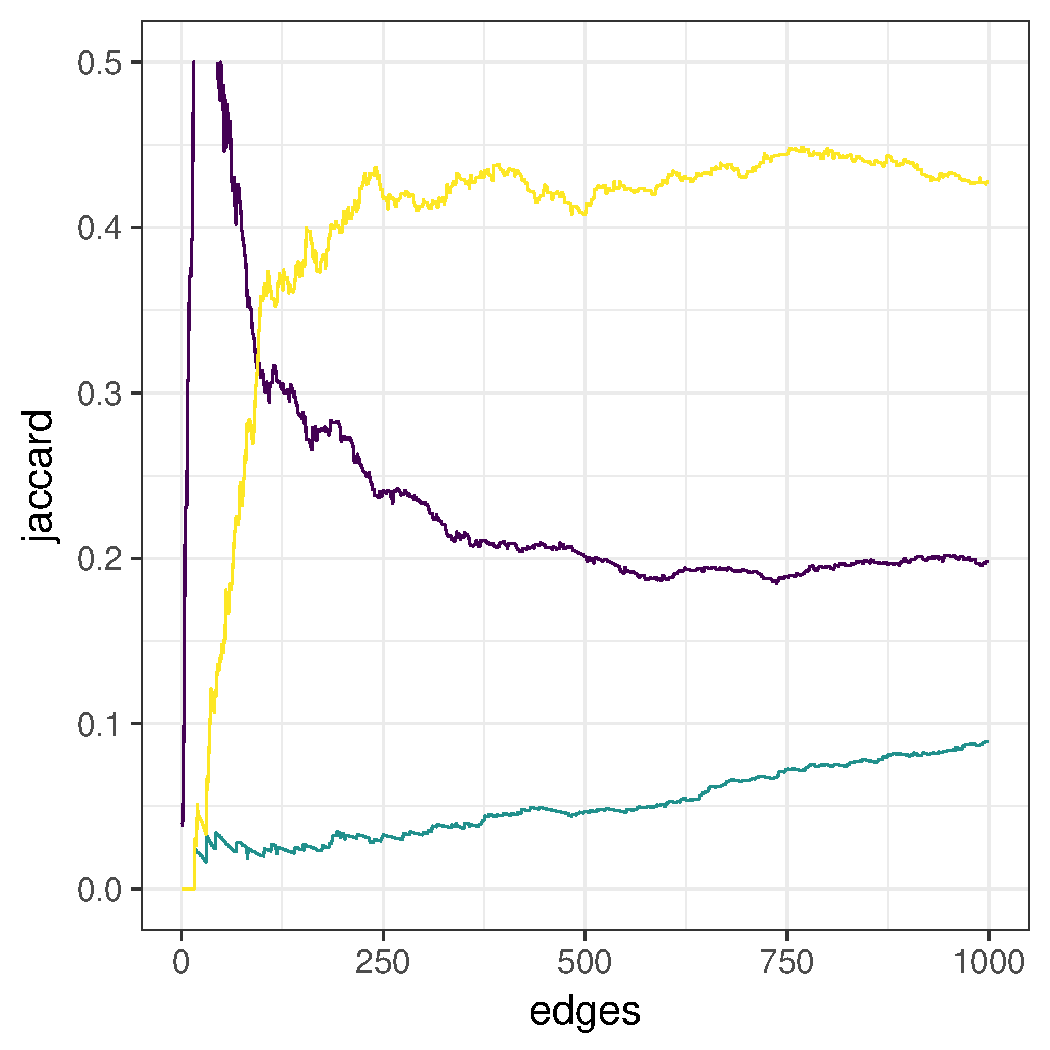
\includegraphics[width=.35\textwidth]{figures/jaccard_RATHER}
  & 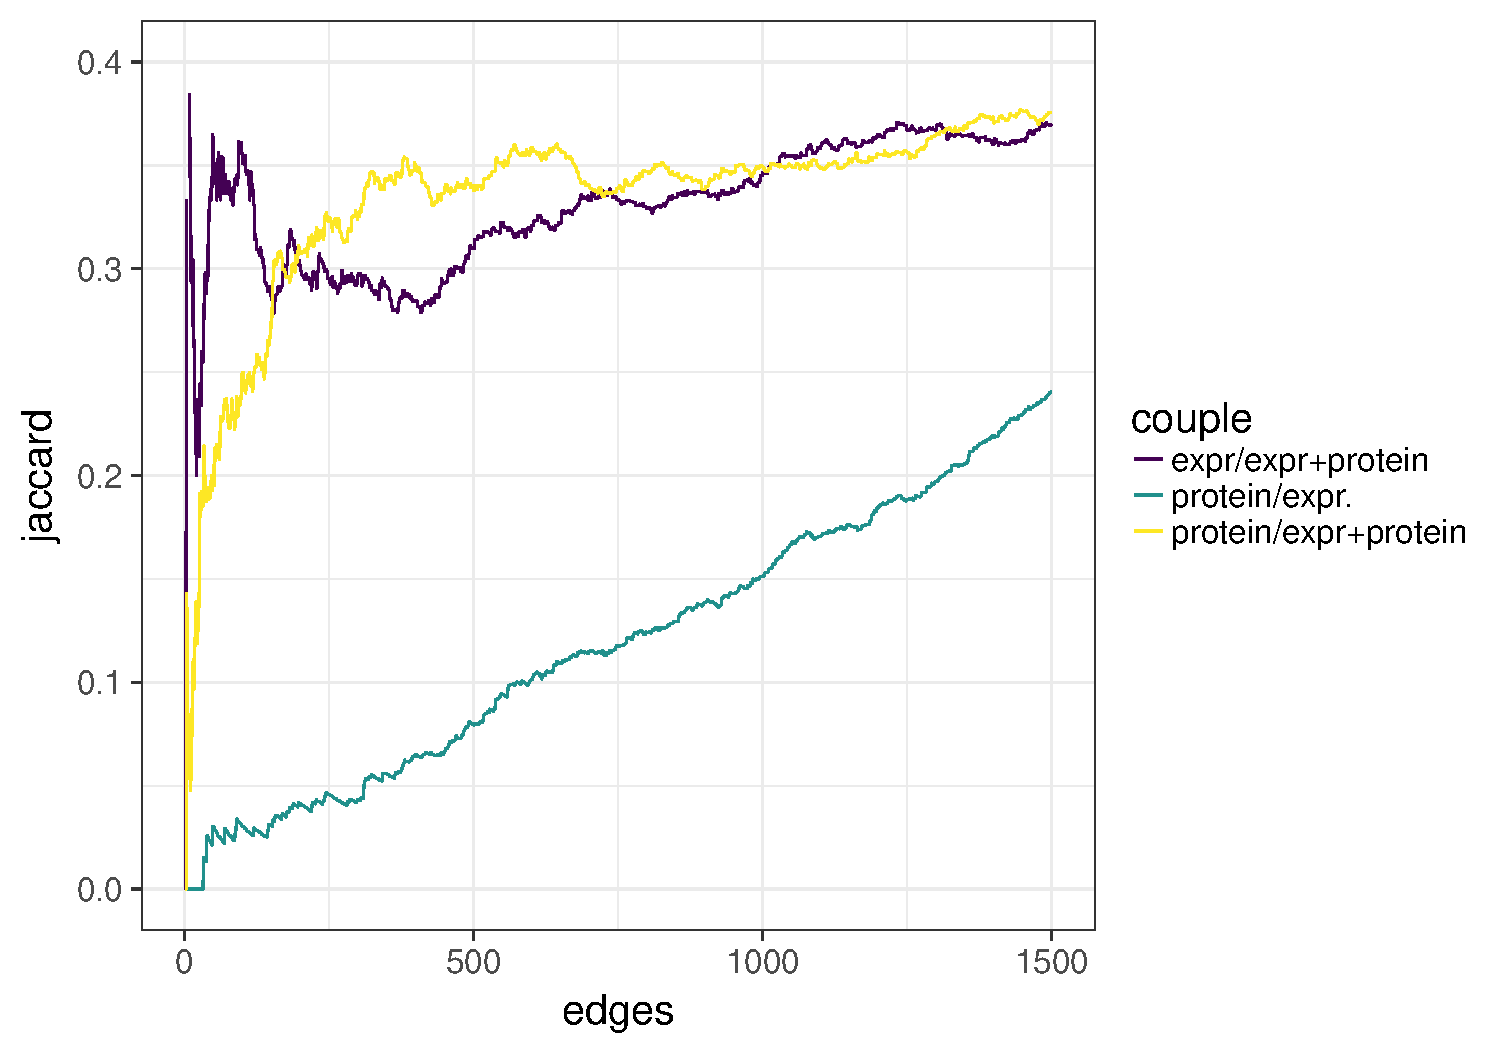
\includegraphics[width=.5\textwidth]{figures/jaccard_NCI60}
  \end{tabular}
  \caption{Jaccard's similarity index
    $J(A,B) = \frac{\left|A\cap B\right|}{\left|A\cup B\right|}$
    between uni-attribute and multiattribute networks, for RATHER and
    NCI60 data set: multiattribute networks share a high Jaccard
    index with both uni-attribute networks.}
  \label{fig:jaccard}
\end{figure}

Figure \ref{fig:networks} shows the finally retained networks, where
the number of edges is controlled by the tuning parameter $\lambda$
chosen by 10-fold cross-validation. It is clear that some motifs only
present in each uni-attribute networks are caught in their
multiattribute counterparts. This tends to prove that the
multiattribute version proposes a consensus version of the
interactions at hand in the cell, and one which is hopefully more
robust to noise.
\begin{figure}[htbp!]
  \centering
  \begin{tabular}{@{}lccc@{}}
    & proteomic network  & genomic network  & multiattribute network \\
    \rotatebox{90}{\hspace{1.2cm}NCI60} 
    & 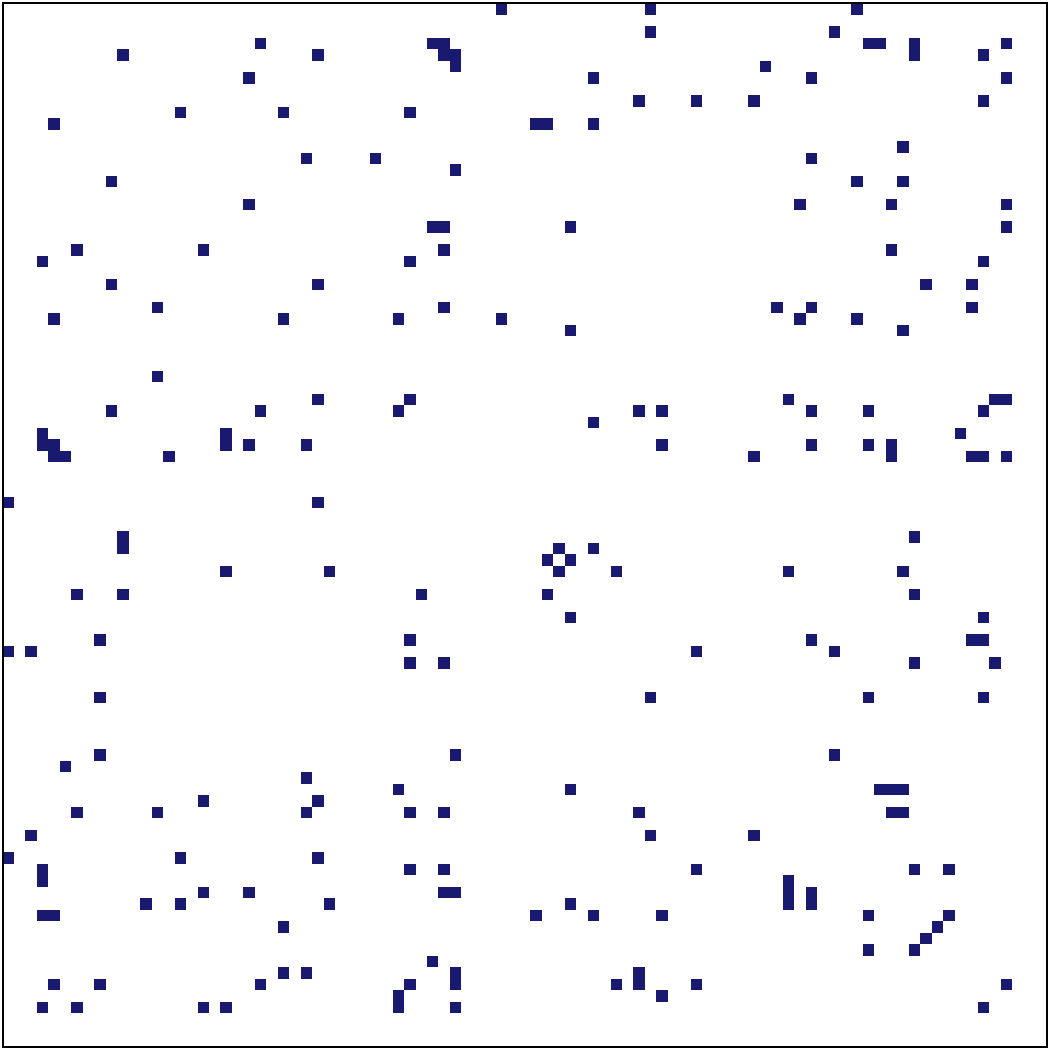
\includegraphics[width=.3\textwidth]{figures/protNet_NCI60}
    & 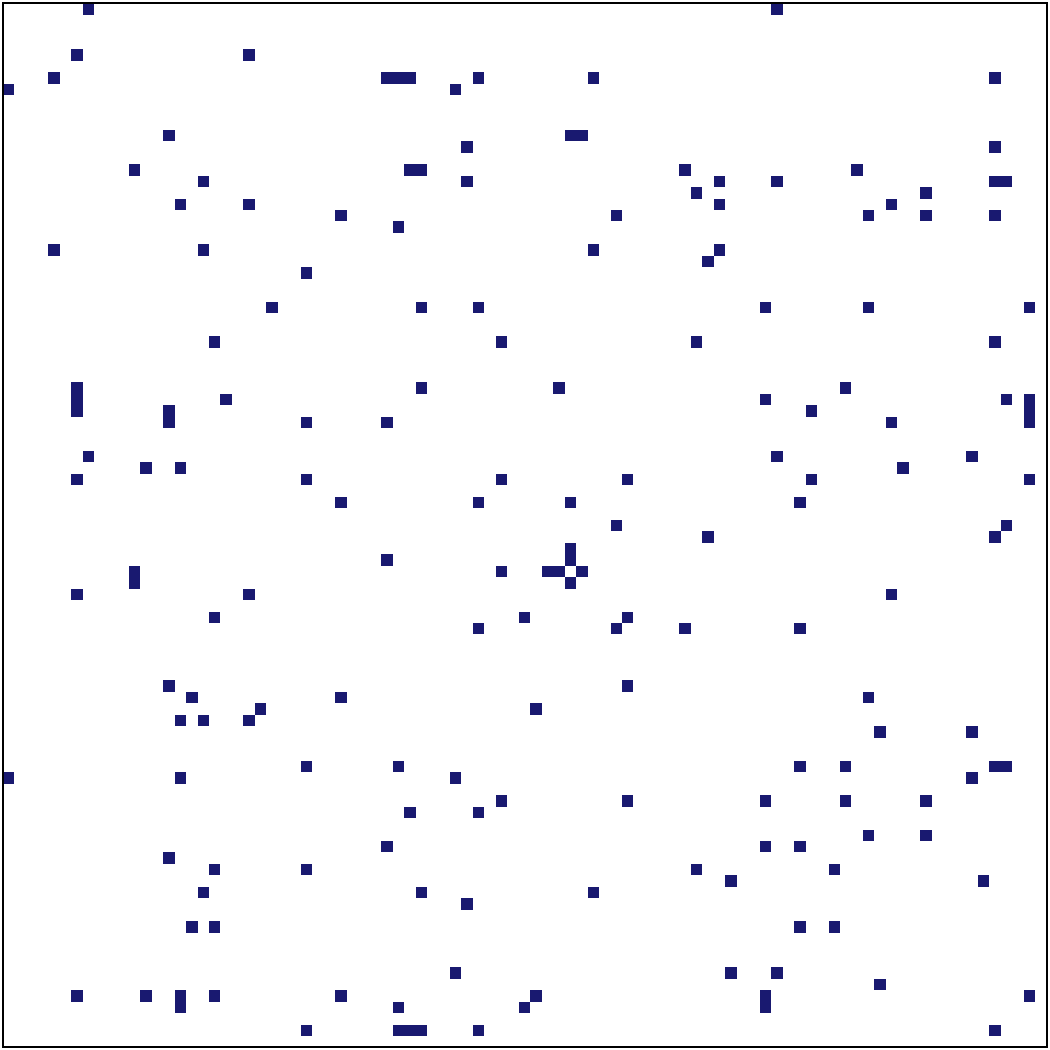
\includegraphics[width=.3\textwidth]{figures/exprNet_NCI60}
    & 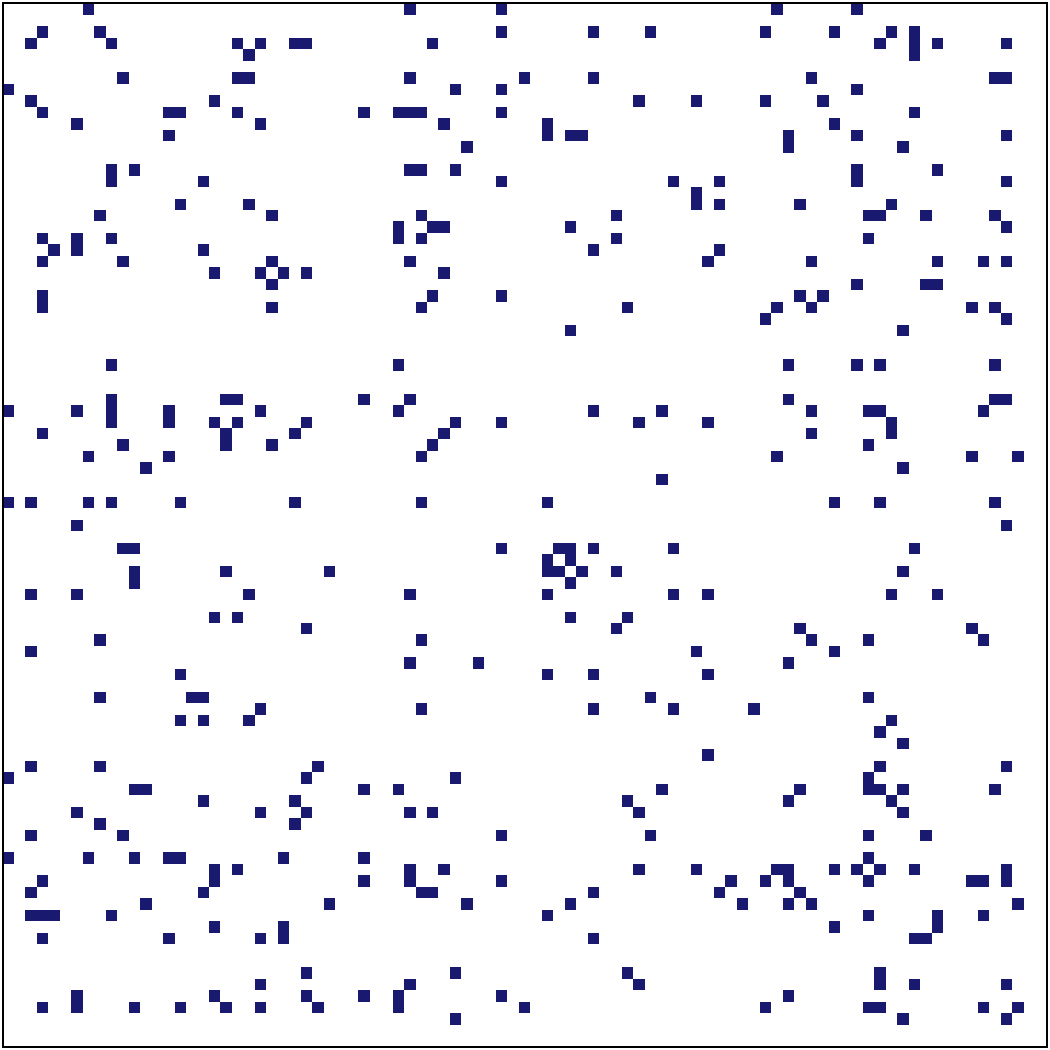
\includegraphics[width=.3\textwidth]{figures/bivarNet_NCI60} \\
    \rotatebox{90}{\hspace{1.2cm}RATHER} 
    & 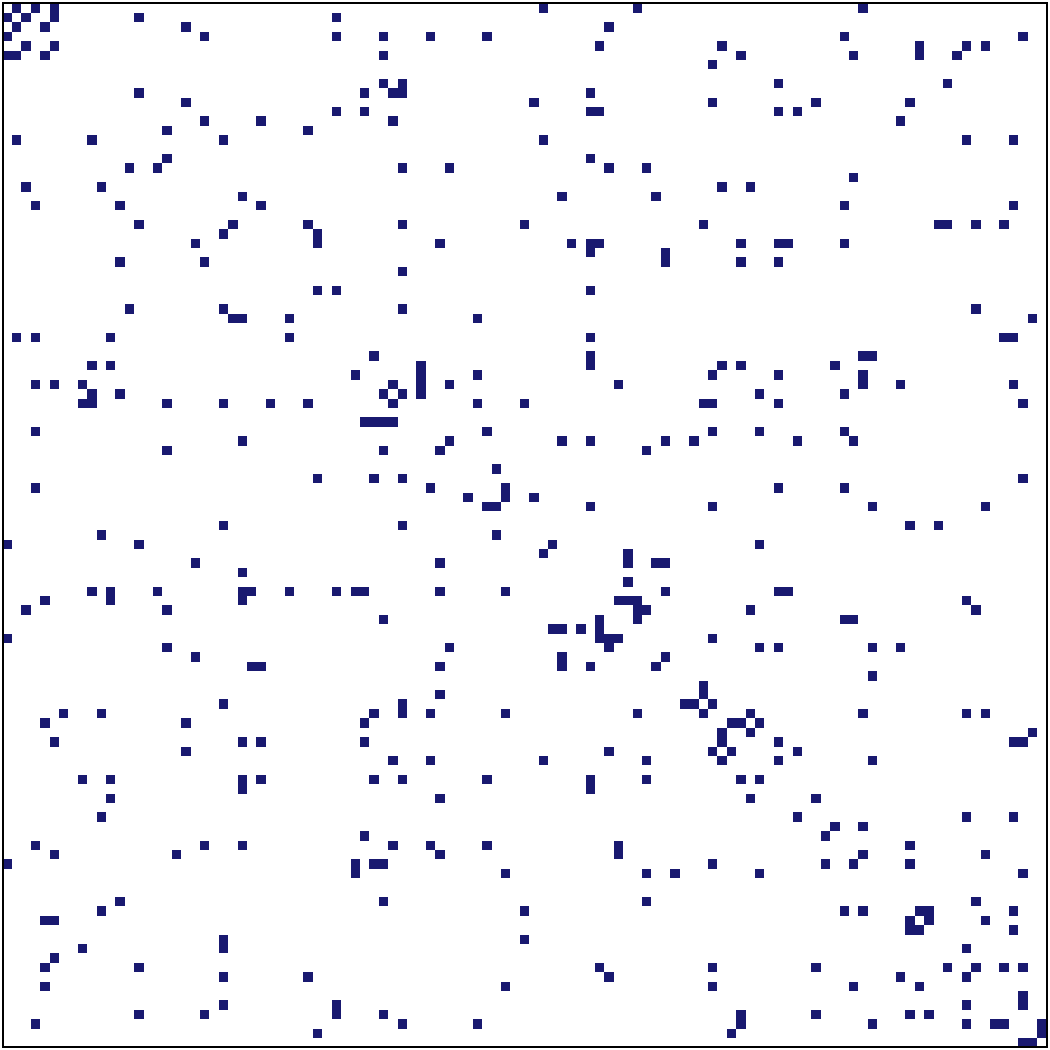
\includegraphics[width=.3\textwidth]{figures/protNet_RATHER}
    & 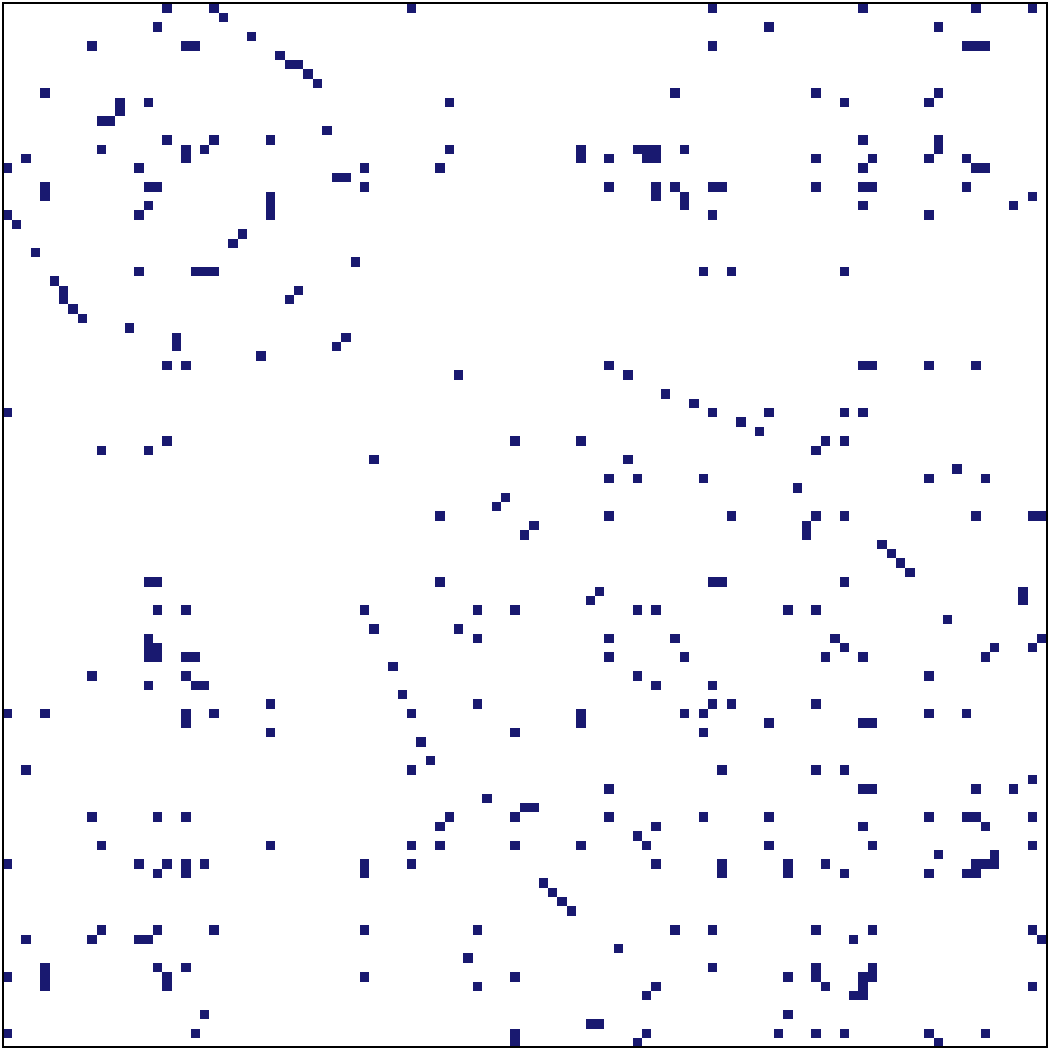
\includegraphics[width=.3\textwidth]{figures/exprNet_RATHER}
    & 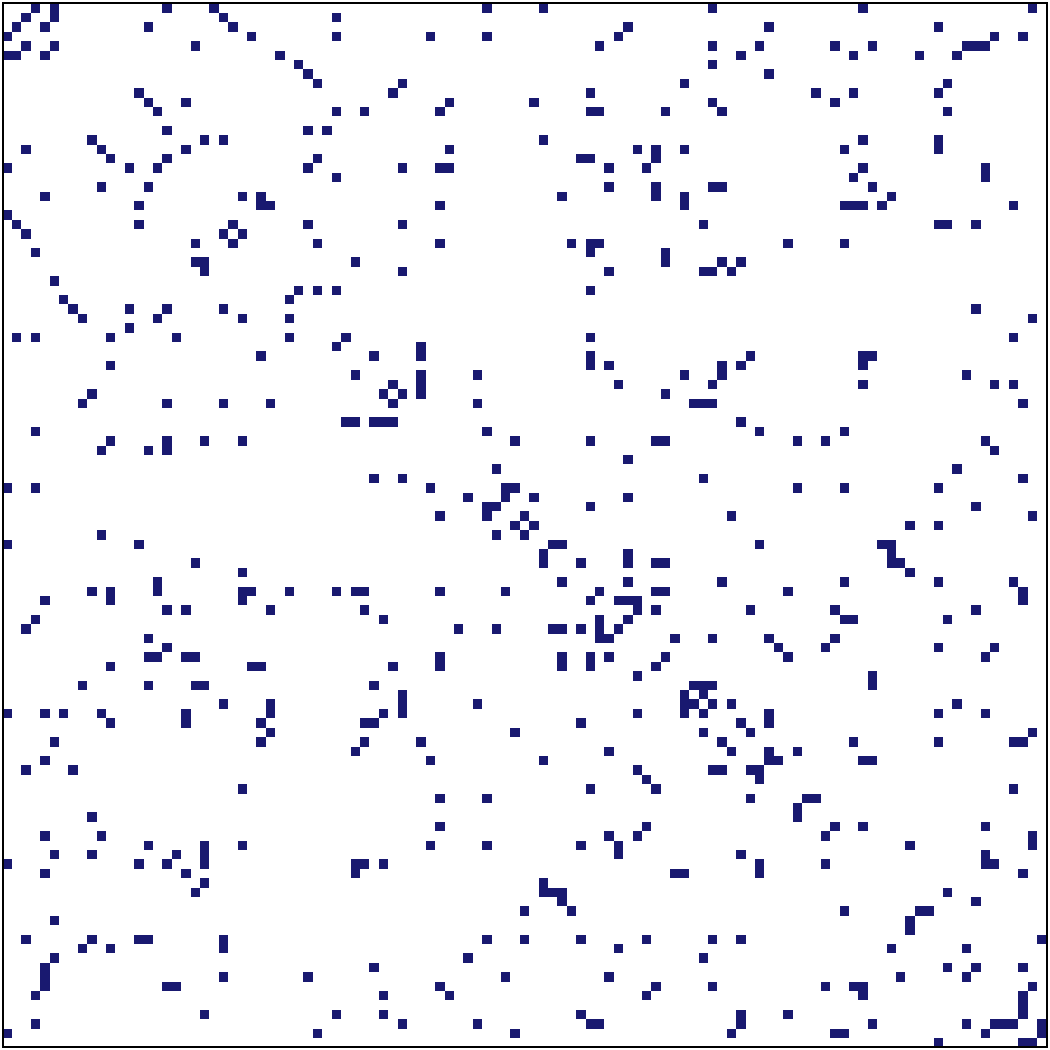
\includegraphics[width=.3\textwidth]{figures/bivarNet_RATHER} \\
  \end{tabular}
  \caption{Uni-attribute and multiattribute networks inferred on both
    NCI60 and RATHER dataset. The number of neighbors of each entity
    is chosen by cross-validation. Multiattribute networks catch motif
    found in the uniattribute counterparts.}
  \label{fig:networks}
\end{figure}






\frame{ \frametitle{Conclusion}

  \paragraph{Perspectives}
  \begin{itemize}
   \item Validation?
   \item Other penalties?
   \item Covariates?
  \end{itemize}
  \medskip

  \begin{block}{\Large\alert{Thanks  to you}  for  your patience  and to  my
    co-workers}
   \end{block}
}

 
% \begin{frame}[allowframebreaks]
%  \frametitle{References}
%   \begin{tiny}
%   \printbibliography
%   \end{tiny}
% \end{frame}

\end{document}

